
\documentclass[journal,fleqn]{IEEEtran}

\usepackage[utf8]{inputenc}
\usepackage[T1]{fontenc}
\usepackage{lmodern}
\usepackage{textcomp}
\usepackage{cite}
\usepackage{amsmath,amssymb,amsfonts,bm,mathtools}
\setlength{\mathindent}{0pt}
\usepackage{graphicx}
\graphicspath{{figs/}{figures/}}
\DeclareGraphicsExtensions{.pdf,.png,.jpg,.jpeg}
\usepackage{booktabs}
\usepackage{multirow}
\usepackage{array}
\usepackage{tabularx}
\usepackage{makecell}
\usepackage{adjustbox}
\usepackage{stfloats}
\usepackage{siunitx}
\usepackage{xcolor}
\usepackage{xurl}
\usepackage[hidelinks]{hyperref}

\newcolumntype{Y}{>{\raggedright\arraybackslash}X}
\renewcommand{\arraystretch}{1.08}
\sisetup{group-separator={,},group-minimum-digits=4,detect-all=true}

\begin{document}


\title{Retrofit Depth vs. Roof-Capped PV in Cooling-Dominated Commercial Buildings: A Techno-Economic Crossover Framework}

\author{Eyas~Khalid~Almughamsi and Marwan~Saleh~Nasser%
\thanks{E. K. Almughamsi and M. S. Nasser are with the Department of Electrical Engineering, College of Engineering, Islamic University of Madinah, Madinah, Saudi Arabia.}%
}

\maketitle

\begin{abstract}

Commercial buildings in hot--humid coastal climates allocate competing capital between energy-efficiency retrofits and behind-the-meter rooftop photovoltaics (PV); however, two binding constraints frequently absent from existing techno-economic frameworks---a physical roof-derived PV capacity ceiling and a no-export tariff condition---can distort the optimal allocation. This paper develops a coupled, calibrated EnergyPlus--HOMER Pro stage-wise framework to identify the net present cost (NPC)-minimising crossover between cumulative retrofit depth and roof-constrained PV deployment for a 12-floor (ground plus 11 upper floors) commercial building in Jeddah, Saudi Arabia. The calibrated baseline (NMBE = +1.90\%, CV(RMSE) = 7.51\%) satisfies ASHRAE Guideline 14 monthly thresholds and is used to generate hourly demand profiles for five retrofit stages (S0 baseline; S1 lighting rationalisation and controls; S2 operational controls and VFD optimisation; S3 glazing and shading improvements; S4 HVAC efficiency improvement). HOMER Pro re-optimises PV and optional Li-ion battery sizing at each stage subject to a 400 kWp roof cap and a zero sell-back tariff. Three contributions emerge. First, for the studied high floor-area-to-roof-area commercial building, and under the assumed tariff, no-export, and PV-cost conditions, the roof-derived capacity cap is binding across all retrofit depths: the PV optimiser selects maximum feasible deployment at every stage, indicating that PV sizing is effectively decoupled from retrofit depth in this configuration. Second, the NPC-minimising crossover stage occurs at S3, with a cumulative retrofit present-value cost of USD 917,532, yielding a total 25-year NPC of USD 8.21 M, equivalent to a saving of USD 362,919 (4.2\%) relative to the USD 8.57 M baseline. Third, the deeper HVAC plant upgrade (S4, CAPEX USD 2.70 M) is shown to require a grid tariff of USD 0.194/kWh---approximately 128\% above the effective Saudi commercial tariff used in this study---to attain NPC neutrality, providing a directly applicable tariff-threshold decision criterion. Battery storage is not selected at any stage, with total PV curtailment remaining below 2.6\% of annual PV generation.

\end{abstract}

\begin{IEEEkeywords}

building energy retrofit; commercial buildings; EnergyPlus; HOMER Pro; net present cost; rooftop photovoltaics; Saudi Arabia; techno-economic optimisation.

\end{IEEEkeywords}

\begin{table*}[!t]
\caption{Nomenclature and Abbreviations Used in This Paper}
\label{tab:01}
\centering
\footnotesize
\setlength{\tabcolsep}{4pt}
\renewcommand{\arraystretch}{1.16}
\begin{tabularx}{\textwidth}{@{}>{\raggedright\arraybackslash}p{0.22\textwidth}>{\raggedright\arraybackslash}X@{}}
\toprule
\textbf{Abbreviation} & \textbf{Definition} \\
\midrule
AHU & Air Handling Unit \\
BMS & Building Management System \\
CAPEX & Capital Expenditure \\
COP & Coefficient of Performance \\
CV(RMSE) & Coefficient of Variation of the Root Mean Square Error \\
EUI & Energy Use Intensity \\
FCU & Fan Coil Unit \\
GCR & Ground Coverage Ratio (PV array) \\
NMBE & Normalized Mean Bias Error \\
NPC & Net Present Cost \\
O\&M & Operation and Maintenance \\
PV & Photovoltaic \\
SAT & Supply Air Temperature \\
SEC & Saudi Electricity Company \\
SHGC & Solar Heat Gain Coefficient \\
UPWF & Uniform Present Worth Factor \\
VFD & Variable Frequency Drive \\
WWR & Window-to-Wall Ratio \\
\bottomrule
\end{tabularx}
\end{table*}

\section{Introduction}

Commercial buildings account for a substantial share of electricity consumption in many economies, with space cooling typically dominating end-use demand in hot climates \cite{ref01}. At the same time, the rapid expansion of renewable electricity technologies strengthens the relevance of behind-the-meter PV as a building-level decarbonisation option \cite{ref02}. Building owners in such regions face a recurring capital-allocation question: should available investment be directed toward energy-efficiency retrofits that reduce demand, or toward behind-the-meter rooftop photovoltaic (PV) systems that offset grid purchases? While this trade-off has been widely investigated under conventional net-metering assumptions, two practical constraints often complicate it in real installations---limited usable roof area and restricted or absent grid export.


In multi-storey commercial buildings, the usable roof footprint is typically much smaller than the total conditioned floor area. Consequently, PV capacity scales with the roof footprint, whereas electricity demand scales with the number of occupied floors. This produces a structural imbalance whereby rooftop PV can offset only a limited fraction of annual electricity demand even when the PV system itself is economically attractive \cite{ref03,ref04}. Where export compensation is unavailable, PV value is realised mainly through self-consumption and avoided grid purchases \cite{ref05}. In parallel, roof-area suitability remains a key physical constraint for rooftop solar applications and can limit the deployable PV capacity in dense building forms \cite{ref06}. Under this no-export condition, retrofit measures alter not only annual demand but also the hourly alignment between building load and PV generation, which in turn affects self-consumption and curtailment.


Previous studies have addressed commercial retrofit packages \cite{ref07,ref08}, building automation and control strategies in cooling-dominated climates \cite{ref09,ref10,ref11}, envelope retrofits in Gulf climates \cite{ref12,ref13}, calibrated whole-building simulation \cite{ref14,ref15}, and PV lifecycle economics \cite{ref05,ref16}. In addition, future electricity-tariff design has been identified as an important factor affecting the economic value of distributed energy resources and demand-side investments \cite{ref17}. The Saudi Building Code SBC 601 \cite{ref18} and ASHRAE Standard 90.1 \cite{ref19} further provide prescriptive baselines for envelope and HVAC performance. However, comparatively few studies explicitly couple calibrated stage-wise hourly demand profiles with constrained PV re-sizing under both a hard roof-cap and a no-export rule. This gap is relevant to the Saudi built environment, where cooling-dominated demand, regional energy-code requirements, and electricity-tariff conditions can affect retrofit economics \cite{ref20,ref21}. It is also directly relevant to office and commercial buildings in Saudi Arabia, where envelope-related retrofit decisions have been shown to influence energy performance \cite{ref12}.


This paper addresses the gap through an EnergyPlus--HOMER Pro framework applied to a multi-storey commercial building in Jeddah, Saudi Arabia. The specific contributions are: (i) a reproducible coupled framework that links calibrated hourly demand profiles with constrained PV--battery optimisation across cumulative retrofit stages; (ii) evidence that, for the studied building geometry and under the assumed tariff and cost conditions, the roof-derived 400 kWp PV capacity cap remains binding across all retrofit depths, effectively decoupling PV sizing from retrofit depth; (iii) identification of Stage 3 as the NPC-minimising retrofit crossover stage, with a cumulative retrofit present-value cost of USD 917,532 and total 25-year NPC savings of USD 362,919 (4.2\% relative to baseline); and (iv) an analytical break-even tariff expression demonstrating that major HVAC plant replacement requires a grid tariff of approximately USD 0.194/kWh---about 128\% above the current commercial tariff---to reach NPC neutrality.


\section{Methodology}

\subsection{Framework Overview and Crossover Criterion}

Fig. 1 illustrates the six-step workflow used to identify the NPC-minimising retrofit crossover stage. Hourly building electricity demand profiles for five scenarios---the baseline case S0 and four cumulative retrofit stages S1--S4---are produced using a calibrated EnergyPlus model. The resulting profiles are imported into HOMER Pro, which evaluates the cost-minimising PV--grid--storage configuration for each stage subject to the same roof-derived PV upper bound. The total 25-year lifecycle NPC is then obtained by combining the HOMER-optimised energy-system NPC with the cumulative present value of retrofit package costs. The analysis evaluates a fixed cumulative retrofit pathway (A $\rightarrow$ B $\rightarrow$ C $\rightarrow$ D) and identifies the NPC-minimising stopping point along this predefined sequence. It does not claim that the identified crossover stage is globally optimal among all possible package combinations; rather, it determines the point at which further deepening of the predefined pathway ceases to be economically justified.


Retrofit costs are not embedded in the HOMER system NPC; they are added externally to obtain the total lifecycle NPC, as detailed in Section II-G. The total NPC at each stage is defined as in (1):


\begin{equation}\label{eq:npc-total}\mathrm{NPC}_{\mathrm{total}}(S_i)=\mathrm{NPC}_{\mathrm{HOMER}}(S_i)+\mathrm{NPC}_{\mathrm{retrofit}}(S_i)\end{equation}

where NPCHOMER(Si) is the 25-year HOMER system NPC for stage i, and NPCretrofit(Si) is the cumulative present value of all retrofit package capital, O\&M, and replacement costs applied up to and including stage i, discounted at a real rate r = 6\% over a 25-year project lifetime.


The NPC-minimising crossover stage S* is then defined as in (2):


\begin{equation}\label{eq:crossover}S^{*}=\arg\min_{S_i\in\{S_0,S_1,S_2,S_3,S_4\}}\mathrm{NPC}_{\mathrm{total}}(S_i)\end{equation}

The no-export condition is enforced by setting the grid sell-back tariff to USD 0.00/kWh; surplus PV electricity is therefore treated as non-compensated curtailable energy in the NPC calculation, with no export revenue contributed in any scenario. Stage-to-stage incremental NPC, used to identify the crossover boundary, is defined in (3):


\begin{equation}\label{eq:delta-npc}\Delta\mathrm{NPC}_{i}=\mathrm{NPC}_{\mathrm{total}}(S_i)-\mathrm{NPC}_{\mathrm{total}}(S_{i-1})\end{equation}

The crossover stage is taken as the stage with the minimum total NPC. For an ordered cumulative retrofit pathway, the crossover boundary is additionally signalled by the first positive $\Delta$NPC following a sequence of negative increments. Results for all five stages are decomposed into HOMER and retrofit components in Table XI, where S* is identified.

\begin{figure*}[!t]
\centering
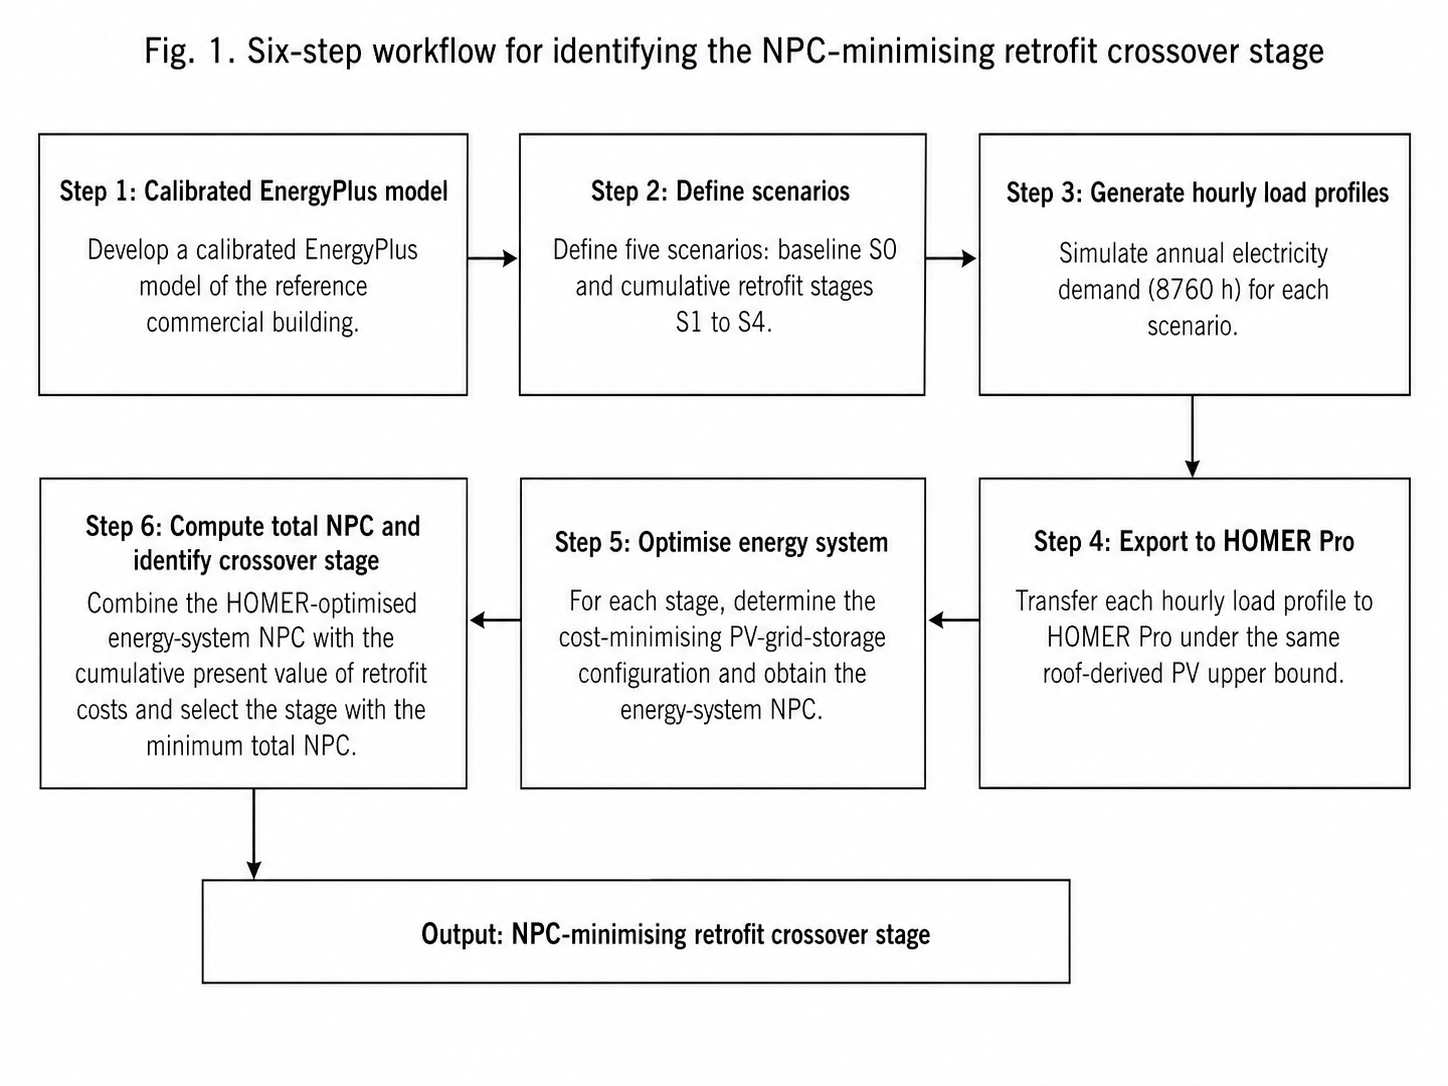
\includegraphics[width=0.95\textwidth]{figs/Fig01.png}
\caption{Proposed EnergyPlus--HOMER Pro workflow for evaluating retrofit stages and identifying the NPC-minimising crossover stage.}
\label{fig:workflow}
\end{figure*}

\subsection{Definition of Retrofit Stages}

To support clear interpretation of the crossover analysis, the five retrofit scenarios are summarised in Table II. The baseline scenario S0 represents the as-operated commercial building before any energy-efficiency intervention and serves as the reference case against which all subsequent stages are compared. Stages S1--S4 are then defined cumulatively: each stage applies the previous stage's measures plus one additional retrofit package, so that S4 contains the full set of measures. This cumulative structure prevents double-counting of savings and makes the marginal contribution of each package directly observable in the simulation results.


\begin{table*}[!t]
\caption{Definition of Retrofit Stages}
\label{tab:02}
\centering
\footnotesize
\setlength{\tabcolsep}{4pt}
\renewcommand{\arraystretch}{1.16}
\begin{tabularx}{\textwidth}{@{}>{\centering\arraybackslash}p{0.10\textwidth}>{\raggedright\arraybackslash}p{0.25\textwidth}>{\raggedright\arraybackslash}X@{}}
\toprule
\textbf{Stage} & \textbf{Designation} & \textbf{Cumulative Scope} \\
\midrule
S0 & Baseline Scenario & As-operated building used as the reference case for all comparisons (no retrofit applied). \\
S1 & Lighting Rationalisation and Controls & S0 + lighting power density rationalisation, occupancy sensors, and lighting-schedule optimisation. \\
S2 & Operational Controls and VFD Optimisation & S1 + AHU fractional availability scheduling, supply-air-temperature reset, and air-side variable-frequency drive (VFD) optimisation. \\
S3 & Glazing and Shading Improvements & S2 + solar-control window film and external fixed shading on the glazed façade. \\
S4 & Full Chiller Plant Replacement and HVAC Efficiency Improvement & S3 + full replacement of the existing chiller plant over the full 2,700 TR installed capacity, represented by improved chiller COP, condenser-fan power reduction, chilled-water-pump VFD operation, and AHU-fan efficiency improvement. \\
\bottomrule
\end{tabularx}
\end{table*}

\noindent{\footnotesize\emph{Note: Each stage is cumulative; stage Si contains the measures of stage Si-1 plus one additional retrofit package, so that S4 represents the deepest retrofit. The corresponding package economics and modelled parameter changes are summarised in Section II-D and Table III.}}\par

\subsection{Demand Modelling and Calibration}

A whole-building electricity demand model was developed in DesignBuilder, which acts as the graphical modelling interface to the EnergyPlus simulation engine \cite{ref22}. EnergyPlus is responsible for solving the building thermal balance and computing HVAC, lighting, equipment, and total electricity demand. The simulation boundary was aligned with the whole-building electricity billing boundary used by the Saudi Electricity Company (SEC) so that measured and simulated electricity consumption are directly comparable.


The baseline demand model was calibrated against twelve consecutive months of whole-building monthly electricity totals. Calibration acceptability was evaluated using the normalized mean bias error (NMBE) and the coefficient of variation of the root mean square error, CV(RMSE), as defined in (4) and (5), following the monthly calibration criteria of ASHRAE Guideline 14 \cite{ref23}:


\begin{equation}\label{eq:nmbe}\mathrm{NMBE}=\left[\frac{\sum(E_{\mathrm{meas},t}-E_{\mathrm{sim},t})}{(n-p)\,\bar{E}_{\mathrm{meas}}}\right]\times100\end{equation}

\begin{equation}\label{eq:cvrmse}\mathrm{CV(RMSE)}=\left[\frac{\sqrt{\sum(E_{\mathrm{meas},t}-E_{\mathrm{sim},t})^2/(n-p)}}{\bar{E}_{\mathrm{meas}}}\right]\times100\end{equation}

where Emeas,t is the measured electricity consumption for month t, Esim,t is the simulated electricity consumption for month t, $\bar{E}$meas is the mean measured monthly consumption, n is the number of monthly calibration points, and p is the number of adjusted calibration parameters. The accept-criteria adopted are |NMBE| $\leq$ 5\% and CV(RMSE) $\leq$ 15\%, in accordance with the monthly thresholds of ASHRAE Guideline 14 \cite{ref23}.


EnergyPlus simulations used a representative Jeddah weather file derived from NASA POWER data \cite{ref24}; the same calibrated model, weather file, occupancy schedules, and operating assumptions were applied across all stages so that differences in stage-wise demand profiles reflect only the modelled retrofit-package parameter changes. The calibrated baseline model was then used to generate representative-year 8,760-hour demand profiles for S0 and the four cumulative retrofit stages S1--S4. The hourly profiles were exported for subsequent techno-economic evaluation in HOMER Pro. HOMER solar-resource inputs were drawn from the same NASA POWER dataset, with an annual average global horizontal irradiance of 5.94 kWh/m$^{2}$$\cdot$day and mean air temperature of 29.2 $^{\circ}$C.


Because calibration is based on monthly utility totals, the resulting 8,760-hour profiles are interpreted as simulation-derived representative demand profiles rather than directly validated measured hourly data. The hourly load shapes are therefore subject to uncertainty in occupancy timing, HVAC scheduling, and intra-day load distribution; this limitation is acknowledged in Section V-G.


\subsection{Cumulative Retrofit Packages}

Four retrofit packages are applied cumulatively in a fixed order, with explicit precedence rules to prevent double-counting: each package modifies only parameters within its defined domain, while parameters introduced by upstream packages are held fixed in subsequent stages. Cost assumptions are based on engineering estimates appropriate for local market conditions and expressed in real USD. Table III summarises the package economics; the modelled parameter changes are described below.


Package A (S0 $\rightarrow$ S1) --- LED lighting rationalisation and controls. The normalised lighting power density is reduced from 0.85 to 0.60 W/m$^{2}$ per 100 lux, and peak occupancy lighting-schedule fractions are reduced by approximately 19\%, consistent with the energy-conservation provisions of SBC 601 \cite{ref18} and ASHRAE 90.1 \cite{ref19}.


Package B (S1 $\rightarrow$ S2) --- Operational controls and air-side VFD optimisation. The AHU availability schedule is restructured from binary on/off operation to fractional part-load operation matched to occupancy. Cooling setpoint scheduling and supply air temperature (SAT) reset are also optimised, while selected air-side fans are converted to VFD operation. This package alters not only annual demand but also the simulated hourly load distribution during occupied and cooling-dominated hours.


Package C (S2 $\rightarrow$ S3) --- Glazing and shading improvements. A low-emissivity solar-control window film is applied to the existing double reflective clear glazing system, and fixed external shading is added to the glazed façade. The film reduces the effective glass-pane SHGC from 0.33 to 0.27, the U-value from 2.53 to 2.30 W/m$^{2}$$\cdot$K, and the visible transmittance from 0.58 to 0.50. The window-to-wall ratio (87\%) and frame type are unchanged.


Package D (S3 $\rightarrow$ S4) --- HVAC efficiency improvement. This package represents the full replacement of the existing chiller plant over the full installed cooling capacity of approximately 2,700 TR. In the EnergyPlus model, this replacement is represented by upgrading the effective chiller COP from 2.8 to 3.5, reducing the condenser-fan power ratio from 0.035 to 0.028, converting chilled-water pumping to variable-speed-drive operation with a motor efficiency of 0.93, and improving AHU-fan efficiency to 0.72. The reported CAPEX for Package D is treated as a net replacement cost after deducting the estimated resale/salvage value of the existing chillers. The negative O\&M value reported for Package D in Table III represents expected maintenance savings relative to the ageing baseline chiller plant, not a revenue stream.


\begin{table*}[!t]
\caption{Retrofit Package Economics (25-Year Horizon, 6\% Real Discount Rate)}
\label{tab:03}
\centering
\scriptsize
\setlength{\tabcolsep}{4pt}
\renewcommand{\arraystretch}{1.16}
\begin{adjustbox}{max width=\textwidth}
\begin{tabular}{@{}lccccc@{}}
\toprule
\textbf{Pkg} & \textbf{Description} & \textbf{CAPEX (USD)} & \textbf{O\&M (USD/yr)} & \textbf{PV of O\&M and Replacements (USD)} & \textbf{Total Package PV (USD)} \\
\midrule
A & Lighting rationalisation + controls & 65,000 & 2,000 & 34,269 & 99,269 \\
B & Controls + VFD & 350,000 & 8,000 & 135,745 & 485,745 \\
C & Solar-control glazing film improvement & 320,000 & 0 & 12,518 & 332,518 \\
D & Full chiller plant replacement, net of resale/salvage credit & 2,700,000 & -15,000 & -191,750 & 2,508,250 \\
\bottomrule
\end{tabular}
\end{adjustbox}
\end{table*}

\noindent{\footnotesize\emph{Note: PV = present value. A negative O\&M value denotes net maintenance savings relative to baseline chiller O\&M, not a positive revenue stream.}}\par

\subsection{Roof-Derived PV Capacity Cap}

The maximum PV capacity is determined from the available roof area rather than treated as an unconstrained optimisation variable. The gross roof footprint is 4,500 m$^{2}$, of which 40\% is excluded for rooftop mechanical equipment, water tanks, safety-access pathways, and constructability setbacks. The exclusion is composed of approximately 25\% for rooftop plant and equipment and 15\% for access and setback requirements. These values are used as project-specific engineering assumptions informed by rooftop PV feasibility and roof-area suitability literature \cite{ref04,ref06}. The usable roof area is computed by (6):


\begin{equation}\label{eq:usable-area}A_{\mathrm{usable}}=A_{\mathrm{gross}}(1-f_{\mathrm{exclusion}})\end{equation}

yielding Ausable = 4,500 $\times$ 0.60 = 2,700 m$^{2}$. The roof-derived PV capacity cap is then computed via (7):


\begin{equation}\label{eq:pv-cap}P_{\mathrm{PV,cap}}=A_{\mathrm{usable}}\times\mathrm{GCR}\times\eta_{\mathrm{module}}\times G_{\mathrm{STC}}\end{equation}

where GCR = 0.65 is the ground coverage ratio for fixed-tilt rows at Jeddah latitude (tilt 22.7$^{\circ}$), $\eta$module = 22.5\% is the rated STC module efficiency, and GSTC = 1 kW/m$^{2}$ is the STC reference irradiance. Substituting the values yields PPV,cap = 2,700 $\times$ 0.65 $\times$ 0.225 = 394.9 $\approx$ 400 kWp. The PV array is modelled as fixed-tilt and south-facing, using the HOMER azimuth convention. The 400 kWp roof cap is held constant across all five stages so that NPC differences between stages reflect retrofit-induced demand-profile changes rather than PV deployment changes.


\subsection{HOMER Pro Optimisation Setup}

For each retrofit stage, HOMER Pro \cite{ref25} was used to identify the minimum-NPC PV--grid--storage configuration under the same roof-derived PV capacity cap. PV capacity was searched from 0 to 400 kWp, with a derating factor of 86\% and a fixed tilt of 22.7$^{\circ}$. Battery storage was included as an optional component using a generic Li-ion model, with candidate capacities ranging from 0 to 1,000 kWh; therefore, zero battery capacity was an admissible and reportable optimisation outcome. The converter efficiency was set to 97\%, the maximum allowable annual capacity shortage was constrained to 0\%, and the Cycle Charging dispatch strategy was applied consistently across all stages.


A zero sell-back tariff (USD 0.00/kWh) represents a conservative no-export or zero-sell-back contractual condition, representative of projects where export compensation is unavailable, not approved, or intentionally disabled. Surplus PV generation therefore receives no economic credit in the NPC calculation. Grid purchases are priced at an energy-only tariff of USD 0.085/kWh, corresponding to the Saudi commercial tariff of 0.32 SAR/kWh for monthly consumption above 6,000 kWh, using an exchange rate of 3.75 SAR/USD \cite{ref26}. Fixed charges, demand charges, and taxes are not separately modelled.


Component assumptions are kept constant across stages to ensure comparability. PV capital and replacement costs are USD 800/kWp and USD 700/kWp, respectively, with O\&M of USD 15/kWp$\cdot$yr and a 25-year service life. Converter capital and replacement costs are USD 150/kW each, with zero annual O\&M and a 15-year life. The Li-ion battery capital cost is USD 300/kWh, replacement cost USD 240/kWh, O\&M USD 5/kWh$\cdot$yr, and lifetime 15 years or 6,000 kWh throughput; these assumptions are broadly aligned with recent NREL battery cost-projection literature \cite{ref27}. The project lifetime is 25 years, the nominal discount rate is 6\%, and inflation is set to 0\%, so all results are expressed on a real-discount-rate basis. Retrofit package costs are excluded from the HOMER system NPC and added externally as described in Section II-G.


To support transparent interpretation of PV energy flows and battery non-selection, the following metrics are defined and reported for each stage (Section IV-A, Table X):


\begin{equation}\label{eq:self-consumption}\mathrm{PV\ self\mbox{-}consumption\ ratio}=\frac{E_{\mathrm{PV,onsite}}}{E_{\mathrm{PV,gen}}}\end{equation}

\begin{equation}\label{eq:self-sufficiency}\mathrm{PV\ self\mbox{-}sufficiency\ ratio}=\frac{E_{\mathrm{PV,onsite}}}{E_{\mathrm{load}}}\end{equation}

\begin{equation}\label{eq:curtailment}\mathrm{PV\ curtailment\ ratio}=\frac{E_{\mathrm{curtailed}}}{E_{\mathrm{PV,gen}}}\end{equation}

where EPV,onsite is the annual PV AC energy delivered to the building load (converter AC output minus grid-exported energy), EPV,gen is the annual PV DC production, Eload is the annual building electricity load, and Ecurtailed is the total annual PV energy that receives no economic value, comprising both DC-side excess electricity and AC-side grid exports at the zero sell-back tariff.


\subsection{Total Lifecycle NPC Computation}

The total lifecycle NPC at each retrofit stage is the sum of the HOMER-optimised system NPC and the cumulative present value of all retrofit packages applied at or before that stage, as already defined in (1). The retrofit-package present value at package j is given in (11):


\begin{equation}\label{eq:npc-pkg}\mathrm{NPC}_{\mathrm{pkg}}(j)=\mathrm{CAPEX}_{j}+\mathrm{PV}(\mathrm{O\&M}_{j})+\mathrm{PV}(\mathrm{Replacements}_{j})\end{equation}

Annual O\&M costs are converted to present value using the uniform present worth factor UPWF = 1/CRF = 12.79, where CRF = 0.0782 corresponds to a real discount rate of 6\% and a 25-year project lifetime. Replacement costs are discounted to the base year using (1 + r)-k, where k is the replacement year. All costs are expressed in real USD. Retrofit package salvage values are assumed negligible for Packages A--C. Package D is treated as a net replacement cost after deducting the expected resale/salvage value of the existing chillers, while HOMER handles energy-system residual values internally through its built-in salvage calculation:


\begin{equation}\label{eq:tau-d}\tau^{*}_{D}=\frac{\mathrm{NPC}_{\mathrm{pkg}}(D)}{\Delta E_{\mathrm{grid},D}\times \mathrm{UPWF}}\end{equation}

where $\Delta$Egrid,D = Egrid(S3) - Egrid(S4) is the annual grid-consumption reduction achieved by Package D. Equation (12) is evaluated in Section V-D to determine the tariff level at which the HVAC efficiency package becomes NPC-neutral.


\subsection{Retrofit Cost Estimation Basis}

The retrofit cost assumptions were developed using a range-based engineering estimation procedure rather than adopting fixed values from a single source. For each package, a practical cost range was first established for the relevant equipment, sensors, controls, installation, commissioning, and contingency items. A representative value within each range was then selected based on the actual retrofit boundary and the case-study building scale. Packages A--C are treated as targeted retrofit measures, including lighting controls, operational controls, air-side VFD optimisation, solar-control window film, and external shading. Package D is treated differently: it represents the full replacement of the existing chiller plant, with the reported CAPEX expressed as the net investment cost after deducting the resale/salvage value of the existing chillers. Therefore, the CAPEX values remain consistent with the techno-economic model used in the NPC analysis. The supporting literature ranges are summarised in Table IV; representative item-level breakdowns and corrected package totals are given in Table V; and the cumulative present-value consistency with the NPC results is confirmed in Table VI.


\begin{table*}[!t]
\caption{Literature and Technical References Supporting Package Cost Ranges}
\label{tab:04}
\centering
\footnotesize
\setlength{\tabcolsep}{4pt}
\renewcommand{\arraystretch}{1.16}
\begin{tabularx}{\textwidth}{@{}>{\raggedright\arraybackslash}p{0.15\textwidth}>{\raggedright\arraybackslash}p{0.25\textwidth}>{\raggedright\arraybackslash}X>{\centering\arraybackslash}p{0.08\textwidth}@{}}
\toprule
\textbf{Package} & \textbf{Retrofit Scope} & \textbf{Literature Range Basis} & \textbf{Ref.} \\
\midrule
A --- LED + Controls & Occupancy sensors, lighting relays, low-voltage wiring, programming, testing. & Lighting-control retrofits in commercial buildings typically add USD 0.50--1.00/ft$^{2}$ to project capital cost, depending on system extent and integration with the BMS. & [28] \\
B --- HVAC Controls + VFD & AHU/FCU reprogramming, sensor verification, SAT reset, selected air-side VFDs, BMS graphics, commissioning. & Sensor and controls retrofits with commissioning fall in the USD 0.98--1.34/ft$^{2}$ range, covering labour, programming, balancing, and testing. & [29] \\
B --- Commissioning & Existing-building commissioning (re-commissioning) component. & Median existing-building commissioning costs reported around USD 0.26/ft$^{2}$ across a wide commercial sample. & [30] \\
C --- Solar-control glazing film & Solar-control window film, external fixed shading, installation, façade access, QA. & Installed solar-control films around USD 7.75/ft$^{2}$ (premium); external shading adds fixed fin/bracket cost USD 45--70/linear m. & [31] \\
D --- Full Chiller Plant Replacement & Full replacement of the existing chiller plant over the full 2,700 TR installed capacity, including high-efficiency chillers, pump/fan VFD-related efficiency measures, plant sensors, BMS integration, electrical works, commissioning, and resale/salvage credit for the existing chillers. & Cost ranges for high-efficiency chiller replacement, pump VFDs, sensors, motors, commissioning, and plant integration are documented in DOE/EPA technical guidance. The selected value is treated as net CAPEX after deducting the residual resale/salvage value of the existing chillers. & [32], [33] \\
\bottomrule
\end{tabularx}
\end{table*}

\begin{table*}[!t]
\caption{Item-Level Cost Estimation Summary by Retrofit Package}
\label{tab:05}
\centering
\scriptsize
\setlength{\tabcolsep}{4pt}
\renewcommand{\arraystretch}{1.16}
\begin{tabularx}{\textwidth}{@{}>{\raggedright\arraybackslash}p{0.12\textwidth}>{\raggedright\arraybackslash}X>{\raggedright\arraybackslash}p{0.17\textwidth}>{\raggedright\arraybackslash}p{0.17\textwidth}>{\centering\arraybackslash}p{0.11\textwidth}@{}}
\toprule
\textbf{Package} & \textbf{Representative Cost Items} & \textbf{Quantity Basis} & \textbf{Unit Range (USD)} & \textbf{Total (USD)} \\
\midrule
A --- LED + Controls & Occupancy sensors (240 units); lighting relays (72 points); LED rationalisation (400 fixtures); floor modules (12 floors); installation; programming; testing. & 240 sensors + 72 relays + 400 fixtures + 12 floors & 60--100/sensor; 70--110/relay; 25--45/fixture & 65,000 \\
B --- HVAC Controls + VFD & AHU/FCU reprogramming (500); sensor verification incl. SAT (120); static-pressure + air-side VFDs (40 AHUs); BMS graphics; SAT reset; chiller/pump supervision; commissioning (12 floors); contingency. & 500 AHU/FCU + 40 VFD units + 12 floors & 90--150/AHU; 1,800--2,600/VFD unit; 3,000--4,500/floor (commissioning) & 350,000 \\
C --- Solar-control glazing film & Solar-control film (4,600 m$^{2}$); surface preparation; installation labour; fixed external shading (1,200 lm); brackets/accessories; façade access (12 floors); mock-up/QA; contingency. & 4,600 m$^{2}$ film + 1,200 linear m shading & 18--26/m$^{2}$ (film); 45--70/linear m (shading); 1,300--2,000/floor (access) & 320,000 \\
D --- Full Chiller Plant Replacement & Full replacement of the existing chiller plant with high-efficiency chillers; removal of existing chillers; mechanical/electrical connection works; BMS integration; testing and commissioning; contingency; less resale/salvage value of old chillers. & 25 existing chillers replaced; total installed cooling capacity $\approx$ 2,700 TR & USD 900--1,100/TR net replacement cost after resale/salvage deduction. Selected value: USD 1,000/TR net & 2,700,000 \\
\bottomrule
\end{tabularx}
\end{table*}

\noindent{\footnotesize\emph{Note: Package D is reported as a net replacement cost after deducting the estimated resale/salvage value of the existing chillers. Therefore, the USD 2.7 million value should not be interpreted as a partial replacement cost or as the gross purchase cost of new chillers only.}}\par

\begin{table*}[!t]
\caption{Cumulative Retrofit Cost Consistency Check}
\label{tab:06}
\centering
\scriptsize
\setlength{\tabcolsep}{4pt}
\renewcommand{\arraystretch}{1.16}
\begin{adjustbox}{max width=\textwidth}
\begin{tabular}{@{}lcccc@{}}
\toprule
\textbf{Stage} & \textbf{Packages Applied} & \textbf{Package PV Added (USD)} & \textbf{Cumulative Retrofit PV Cost (USD)} & \textbf{Formula} \\
\midrule
S0 & Baseline & --- & --- & No retrofit cost \\
S1 & A & 99,269 & 99,269 & A \\
S2 & A + B & 485,745 & 585,014 & 99,269 + 485,745 \\
S3 $\star$ & A + B + C & 332,518 & 917,532 & 585,014 + 332,518 \\
S4 & A + B + C + D & 2,508,250 & 3,425,782 & 917,532 + 2,508,250 \\
\bottomrule
\end{tabular}
\end{adjustbox}
\end{table*}

\section{Case Study Application}

\subsection{Building and Tariff Context}

The case-study building is the Bin Homran Commercial Center, a 12-floor (ground floor plus 11 upper floors) office-dominant commercial high-rise in Jeddah, Saudi Arabia (21.75$^{\circ}$N, 39.25$^{\circ}$E). An unconditioned basement car park and a rooftop plant level are excluded from the energy-model boundary. Each conditioned floor has a gross floor area of 4,500 m$^{2}$, yielding a total conditioned area of 54,000 m$^{2}$ and a floor-area-to-roof-area ratio of 12:1. Jeddah experiences a hot--humid coastal climate with an annual mean dry-bulb temperature of 29.2 $^{\circ}$C and global horizontal irradiance of 5.94 kWh/m$^{2}$$\cdot$day. The building is served by a centralised chilled-water HVAC system comprising approximately 500 terminal units (AHUs and FCUs) and 25 modular chillers with combined installed cooling capacity of about 2,700 TR. The envelope consists mainly of a continuous double-glazed curtain-wall façade with a window-to-wall ratio (WWR) of approximately 87\%. In the calibrated baseline model, the glazing properties are represented by a U-value of 2.53 W/m$^{2}$$\cdot$K, an SHGC of 0.33, and a visible transmittance of 0.58. Package C does not change the glass material, curtain-wall geometry, or WWR; instead, it represents the application of solar-control window film and external fixed shading. In the retrofit model, this façade improvement is represented by an effective U-value of 2.30 W/m$^{2}$$\cdot$K, an SHGC of 0.27, and a visible transmittance of 0.50, while the external shading is treated as a façade-level reduction in effective solar gains, and the baseline chiller plant operates at a reference COP of 2.80 with a leaving chilled-water temperature of approximately 5.6 $^{\circ}$C. The occupied cooling setpoint is 24 $^{\circ}$C, with a setback of 28 $^{\circ}$C during unoccupied periods. Energy cost analysis applies an effective Saudi commercial tariff of USD 0.085/kWh, corresponding to 0.32 SAR/kWh for monthly commercial consumption above 6,000 kWh, under a conservative no-export contractual condition in which surplus PV electricity receives no compensation \cite{ref26}.


\subsection{Calibration Results}

The baseline energy model (S0) was developed in DesignBuilder/EnergyPlus using documented building geometry, HVAC configuration, and occupancy schedules derived from facility records, then calibrated against twelve consecutive months of SEC billing data. Calibration acceptability was assessed against the ASHRAE Guideline 14 monthly thresholds (|NMBE| $\leq$ 5\% and CV(RMSE) $\leq$ 15\%) \cite{ref23}; both criteria were satisfied (NMBE = +1.90\%, CV(RMSE) = 7.51\%), confirming the suitability of the baseline as a reference for stage-wise comparison.


Fig. 2 presents the measured versus simulated monthly electricity consumption, and Table VII reports the corresponding monthly residuals. The largest individual monthly deviation occurs in November (-14.3\%), which may reflect atypical occupancy or operational conditions in that month; however, the annual aggregate metrics remain well within the ASHRAE Guideline 14 acceptance criteria. Fig. 3 presents load-duration curves for all five stages (S0--S4), illustrating the progressive reduction in peak and intermediate loads with deeper retrofit application. The calibrated baseline model was then used to generate representative-year hourly demand profiles for S0 and the four cumulative retrofit stages S1--S4, which were subsequently exported to HOMER Pro for PV--grid optimisation under each retrofit scenario.

\begin{figure*}[!t]
\centering
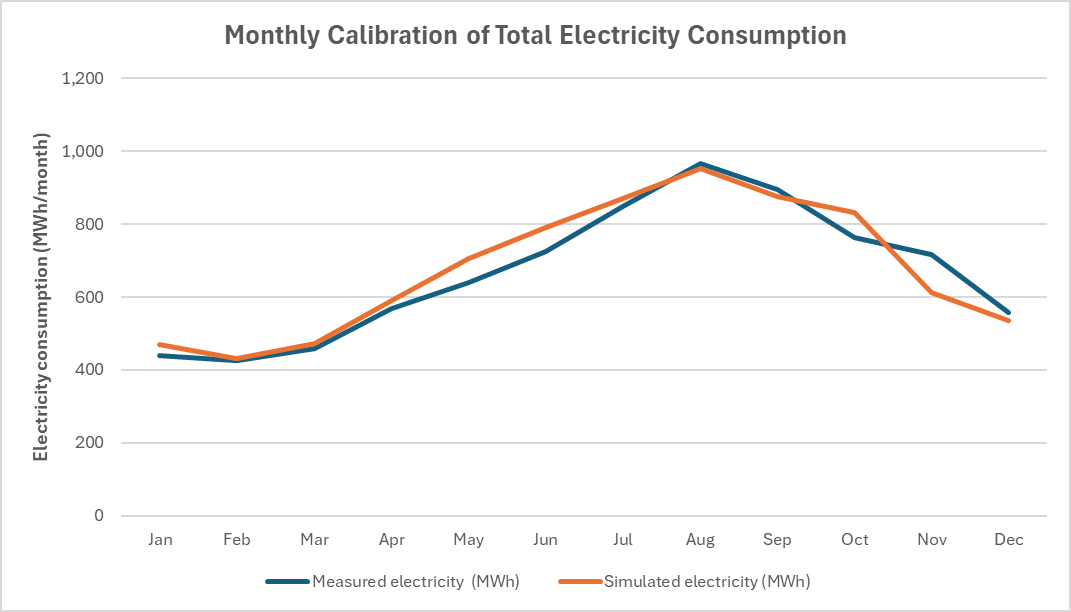
\includegraphics[width=0.75\textwidth]{figs/Fig02.png}
\caption{Measured versus simulated monthly electricity consumption (calibration period).}
\label{fig:calibration}
\end{figure*}

\begin{table*}[!t]
\caption{Monthly Residuals between Measured and Simulated Electricity Consumption}
\label{tab:07}
\centering
\scriptsize
\setlength{\tabcolsep}{4pt}
\renewcommand{\arraystretch}{1.16}
\begin{adjustbox}{max width=\textwidth}
\begin{tabular}{@{}lrrrr@{}}
\toprule
\textbf{Month} & \textbf{Measured (MWh)} & \textbf{Simulated (MWh)} & \textbf{Residual (MWh)} & \textbf{Error (\%)} \\
\midrule
Jan & 438.75 & 470.84 & +32.10 & +7.32 \\
Feb & 425.91 & 430.12 & +4.21 & +0.99 \\
Mar & 458.45 & 472.79 & +14.34 & +3.13 \\
Apr & 569.15 & 591.32 & +22.18 & +3.90 \\
May & 638.87 & 707.05 & +68.18 & +10.67 \\
Jun & 725.35 & 789.83 & +64.48 & +8.89 \\
Jul & 847.20 & 869.27 & +22.07 & +2.61 \\
Aug & 965.58 & 952.93 & -12.65 & -1.31 \\
Sep & 895.39 & 874.85 & -20.55 & -2.29 \\
Oct & 762.58 & 833.16 & +70.57 & +9.25 \\
Nov & 715.59 & 613.26 & -102.33 & -14.30 \\
Dec & 558.57 & 535.66 & -22.91 & -4.10 \\
\bottomrule
\end{tabular}
\end{adjustbox}
\end{table*}

Note: Annual aggregate satisfies ASHRAE Guideline 14 monthly thresholds (NMBE = +1.90\%, CV(RMSE) = 7.51\%).

\begin{figure*}[!t]
\centering
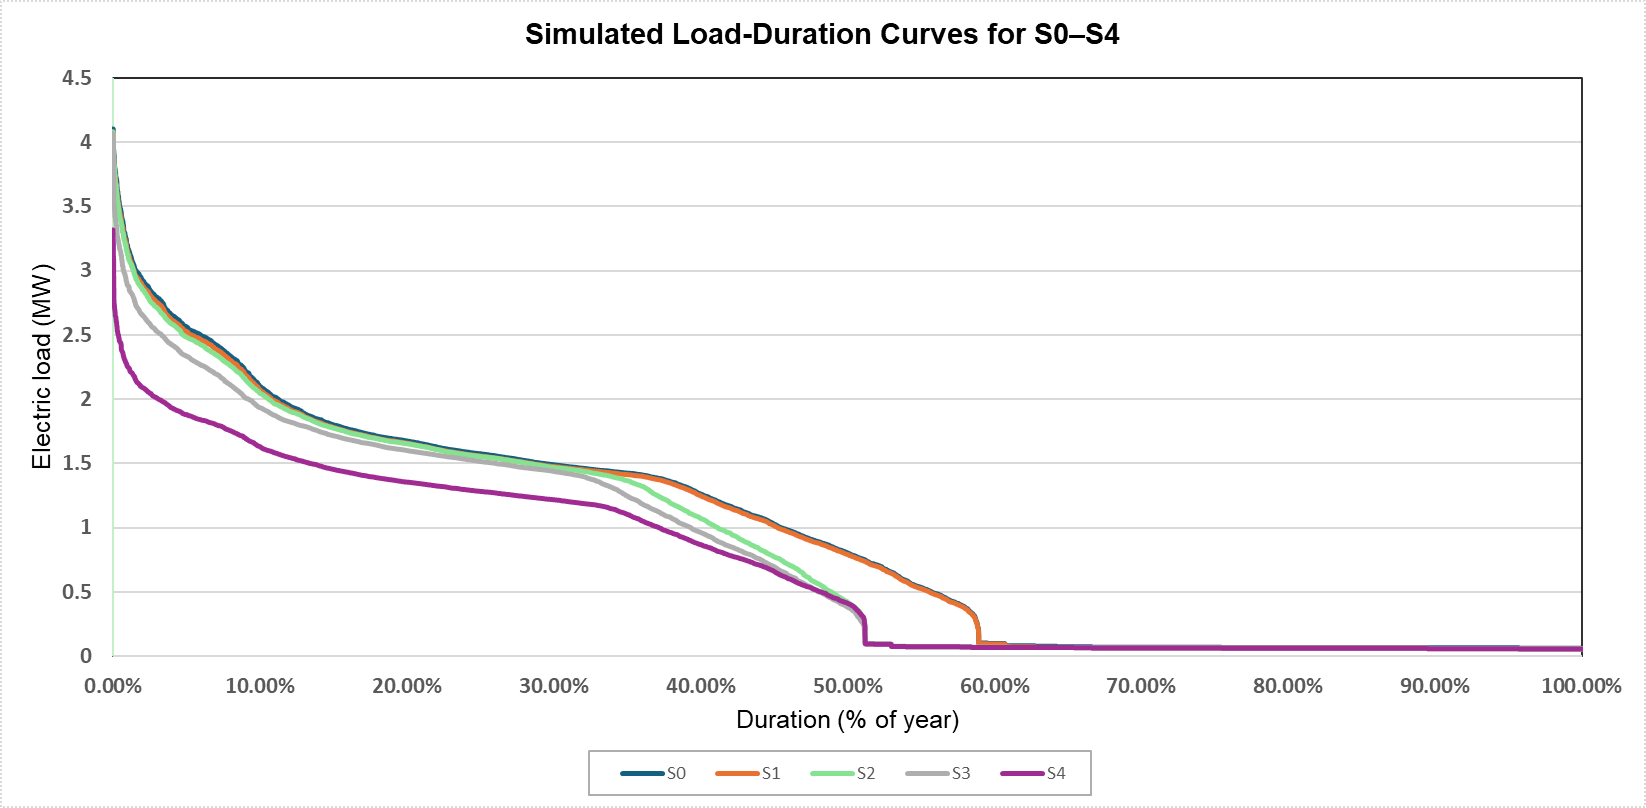
\includegraphics[width=0.95\textwidth]{figs/Fig03.png}
\caption{Simulated load-duration curves for retrofit stages S0--S4.}
\label{fig:load-duration}
\end{figure*}

\subsection{Demand Reduction by Stage}

Table VIII summarises the whole-building annual electricity consumption, EUI, and peak demand for each retrofit stage. The baseline (S0) provides a reference consumption of 8,141,075 kWh/yr (EUI = 150.8 kWh/m$^{2}$$\cdot$yr) and peak demand of 3,940 kW. Marginal reductions range from a modest -1.4\% at S1 (lighting controls) to a cumulative -27.0\% at S4 (full chiller plant replacement and HVAC efficiency improvement), with peak demand declining progressively from 3,940 kW at S0 to 3,082 kW at S4. As discussed in Section IV, however, the high capital intensity of Package D causes S4 to be economically suboptimal relative to S3 once retrofit costs are considered. The hourly profiles for each stage are exported directly to HOMER Pro for techno-economic re-optimisation.


\begin{table*}[!t]
\caption{Annual Electricity Consumption and Peak Demand by Stage}
\label{tab:08}
\centering
\scriptsize
\setlength{\tabcolsep}{4pt}
\renewcommand{\arraystretch}{1.16}
\begin{adjustbox}{max width=\textwidth}
\begin{tabular}{@{}lrrrrr@{}}
\toprule
\textbf{Stage} & \textbf{Packages Applied} & \textbf{Annual Consumption (kWh/yr)} & \textbf{EUI (kWh/m$^{2}$$\cdot$yr)} & \textbf{vs. S0 (\%)} & \textbf{Peak Demand (kW)} \\
\midrule
S0 & Baseline & 8,141,075 & 150.8 & --- & 3,940 \\
S1 & A --- Lighting Controls & 8,031,066 & 148.7 & -1.4 & 3,918 \\
S2 & A+B --- Controls & 7,352,805 & 136.2 & -9.7 & 3,897 \\
S3 & A+B+C --- Glazing & 6,951,987 & 128.7 & -14.6 & 3,862 \\
S4 & A+B+C+D --- HVAC & 5,940,050 & 110.0 & -27.0 & 3,082 \\
\bottomrule
\end{tabular}
\end{adjustbox}
\end{table*}

\section{Results}

\subsection{HOMER Optimisation Results}

Table IX presents the HOMER Pro optimisation results for all five stages. The roof-derived 400 kWp cap is binding at every stage: the optimiser selects exactly 400 kW of PV regardless of retrofit depth or annual demand level, confirming that, for this high floor-area-to-roof-area building and under the assumed tariff, no-export, and PV-cost conditions, PV sizing is effectively decoupled from retrofit depth. Battery storage is not selected at any stage (0 kWh optimal throughout), a result examined analytically in Section V-E. Annual PV output remains constant at 732,958 kWh/yr across stages. The renewable fraction---defined as PV production divided by the sum of PV production and grid purchases---increases from 8.98\% at S0 to 12.26\% at S4 as building demand decreases. HOMER system NPC declines monotonically from USD 8,569,230 at S0 to USD 6,184,868 at S4, reflecting reduced grid purchases at each successive retrofit stage. CO$_{2}$ emissions follow the same trend, falling from 4,697,728 kg/yr at S0 to 3,306,679 kg/yr at S4.


\begin{table*}[!t]
\caption{HOMER Pro Optimisation Results by Stage}
\label{tab:09}
\centering
\scriptsize
\setlength{\tabcolsep}{4pt}
\renewcommand{\arraystretch}{1.16}
\begin{adjustbox}{max width=\textwidth}
\begin{tabular}{@{}cccrcrr@{}}
\toprule
\textbf{Stage} & \textbf{PV (kW)} & \textbf{Battery (kWh)} & \textbf{Grid (kWh/yr)} & \textbf{Renewable Fraction (\%)} & \textbf{HOMER NPC (USD)} & \textbf{CO$_{2}$ (kg/yr)} \\
\midrule
S0 & 400 & 0 & 7,433,492 & 8.98 & 8,569,230 & 4,697,728 \\
S1 & 400 & 0 & 7,323,669 & 9.10 & 8,449,436 & 4,628,202 \\
S2 & 400 & 0 & 6,660,200 & 9.91 & 7,725,722 & 4,199,540 \\
S3 $\star$ & 400 & 0 & 6,259,631 & 10.48 & 7,288,779 & 3,946,224 \\
S4 & 400 & 0 & 5,247,615 & 12.26 & 6,184,868 & 3,306,679 \\
\bottomrule
\end{tabular}
\end{adjustbox}
\end{table*}

\noindent{\footnotesize\emph{Note: Renewable fraction = PV production / (PV production + grid purchases). Annual PV production is 732,958 kWh/yr in all stages because the roof-derived 400 kWp PV cap is binding throughout.}}\par

Table X presents the detailed HOMER energy balance for all five stages, decomposing PV generation into consumed, curtailed, and loss components. The energy-balance decomposition confirms that the roof-capped PV system is small relative to the building load: the PV self-consumption ratio exceeds 94\% at all stages, and the PV self-sufficiency ratio ranges from 8.69\% (S0) to 11.66\% (S4). Total PV curtailment remains below 2.6\% across all stages. At the deepest retrofit (S4), the annual economic value of the curtailed energy is only 18,628 kWh $\times$ USD 0.085/kWh $\approx$ USD 1,583/yr (25-year present value $\approx$ USD 20,247), which is insufficient to justify any battery capacity at current capital costs. This energy-balance evidence underpins the zero-battery HOMER result reported in Table IX and is analysed further in Section V-E.


\begin{table*}[!t]
\caption{HOMER Energy Balance by Retrofit Stage}
\label{tab:10}
\centering
\scriptsize
\setlength{\tabcolsep}{4pt}
\renewcommand{\arraystretch}{1.16}
\begin{adjustbox}{max width=\textwidth}
\begin{tabular}{@{}lrrrrrr@{}}
\toprule
\textbf{Parameter} & \textbf{Unit} & \textbf{S0} & \textbf{S1} & \textbf{S2} & \textbf{S3} & \textbf{S4} \\
\midrule
Annual load served & kWh/yr & 8,141,077 & 8,031,066 & 7,352,805 & 6,951,987 & 5,940,049 \\
PV DC generation & kWh/yr & 732,958 & 732,958 & 732,958 & 732,958 & 732,958 \\
PV AC delivered to load & kWh/yr & 707,585 & 707,397 & 692,605 & 692,356 & 692,434 \\
PV AC exported to grid (at \$0) & kWh/yr & 377 & 565 & 15,357 & 15,606 & 15,528 \\
DC-side excess electricity & kWh/yr & 3,100 & 3,100 & 3,100 & 3,100 & 3,100 \\
Total curtailed PV & kWh/yr & 3,477 & 3,665 & 18,457 & 18,706 & 18,628 \\
Grid purchases & kWh/yr & 7,433,492 & 7,323,669 & 6,660,200 & 6,259,631 & 5,247,615 \\
Inverter/converter losses & kWh/yr & 21,896 & 21,896 & 21,896 & 21,896 & 21,896 \\
Selected battery capacity & kWh & 0 & 0 & 0 & 0 & 0 \\
Renewable fraction & \% & 8.98 & 9.10 & 9.91 & 10.48 & 12.26 \\
PV self-consumption ratio & \% & 96.54 & 96.51 & 94.49 & 94.46 & 94.47 \\
PV self-sufficiency ratio & \% & 8.69 & 8.81 & 9.42 & 9.96 & 11.66 \\
PV curtailment ratio & \% & 0.47 & 0.50 & 2.52 & 2.55 & 2.54 \\
\bottomrule
\end{tabular}
\end{adjustbox}
\end{table*}

\noindent{\footnotesize\emph{Note: PV AC delivered to load = converter AC output - grid exports. Total curtailed PV = DC-side excess + grid exports (both receive zero economic value under the no-export condition). Renewable fraction = PV DC generation / (PV DC generation + grid purchases). Definitions of self-consumption, self-sufficiency, and curtailment ratios are given in (8)--(10).}}\par

\subsection{Total Lifecycle NPC Analysis and Crossover Identification}

Table XI combines the HOMER system NPC with the cumulative present value of retrofit package costs to determine the total lifecycle NPC at each stage. The NPC-minimising crossover is clearly identified at S3, with a total NPC of USD 8,206,311---a saving of USD 362,919 (4.2\%) relative to the USD 8,569,230 baseline. This identifies S3 as the NPC-minimising stopping point along the predefined cumulative retrofit pathway, under the modelled tariff, cost, and roof-availability assumptions.


\begin{table*}[!t]
\caption{Total Lifecycle NPC and Crossover Identification}
\label{tab:11}
\centering
\scriptsize
\setlength{\tabcolsep}{4pt}
\renewcommand{\arraystretch}{1.16}
\begin{adjustbox}{max width=\textwidth}
\begin{tabular}{@{}lrrrrr@{}}
\toprule
\textbf{Stage} & \textbf{HOMER NPC (USD)} & \textbf{Cumulative Retrofit PV Cost (USD)} & \textbf{Total NPC (USD)} & \textbf{$\Delta$NPC vs. S0 (USD)} & \textbf{Decision} \\
\midrule
S0 & 8,569,230 & --- & 8,569,230 & --- & Reference \\
S1 & 8,449,436 & 99,269 & 8,548,705 & -20,525 & Marginal \\
S2 & 7,725,722 & 585,014 & 8,310,736 & -258,494 & Viable \\
S3 $\star$ & 7,288,779 & 917,532 & 8,206,311 & -362,919 & S* (min NPC) \\
S4 & 6,184,868 & 3,425,782 & 9,610,650 & +1,041,420 & Unviable \\
\bottomrule
\end{tabular}
\end{adjustbox}
\end{table*}

The stage-to-stage incremental NPC values ($\Delta$NPCi) are negative through S3, indicating that each of the first three retrofit packages produces a net economic benefit when its full lifecycle cost is included: $\Delta$NPC1 = -USD 20,525 (S0 $\rightarrow$ S1), $\Delta$NPC2 = -USD 237,969 (S1 $\rightarrow$ S2), and $\Delta$NPC3 = -USD 104,425 (S2 $\rightarrow$ S3). The sign of $\Delta$NPC reverses sharply at S3 $\rightarrow$ S4: $\Delta$NPC4 = +USD 1,404,339, marking the crossover boundary. This reversal is driven by the USD 2,508,250 present-value cost of Package D substantially exceeding the corresponding HOMER NPC reduction of USD 1,103,911. The total NPC at S4 reaches USD 9,610,650, which is USD 1,041,420 worse than the unretrofitted baseline. Fig. 4 visualises the 25-year total lifecycle NPC across the five retrofit stages by decomposing each stage into the HOMER-optimised system NPC and the cumulative retrofit present-value cost. The stacked bars show the contribution of each cost component, while the overlaid line represents the resulting total lifecycle NPC. The figure shows that total NPC decreases gradually from S0 to S3, where the minimum value is achieved, before increasing sharply at S4. This confirms that S3 represents the NPC-minimising crossover stage, while the transition from S3 to S4 introduces an economic penalty despite the additional energy savings achieved by the HVAC upgrade package.


\begin{figure*}[!t]
\centering
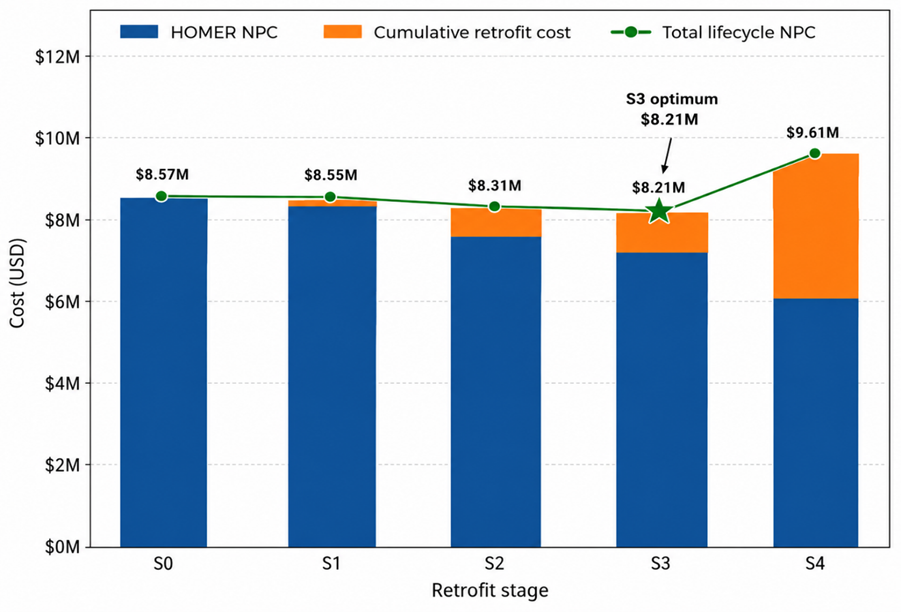
\includegraphics[width=0.78\textwidth]{figs/Fig04.png}
\caption{Decomposition of total 25-year lifecycle NPC by retrofit stage, with S3 identified as the minimum-NPC crossover point.}
\label{fig:npc-crossover}
\end{figure*}

\subsection{Bounded Robustness Assessment}

A bounded robustness assessment was conducted to verify that the NPC-minimising crossover remains stable under selected parameter perturbations. First, PV CAPEX was varied by $\pm$20\%, with the roof cap, tariff, no-export rule, and retrofit costs held constant. The crossover conclusion was unchanged: S3 retained the minimum total NPC under the -20\%, base, and +20\% PV CAPEX cases, with total NPC values of USD 8.14 M, USD 8.21 M, and USD 8.27 M, respectively. HOMER continued to select the full 400 kWp PV capacity in every scenario, confirming that the roof-derived PV cap remains binding across the tested PV-cost range.


Second, Stage 4 was tested against break-even conditions. Relative to S3, S4 requires an effective grid tariff of USD 0.194/kWh ($\approx$ 0.727 SAR/kWh) to become NPC-neutral, or, alternatively, a reduction of approximately USD 1.40 M in the present value of Package D---corresponding to an HVAC CAPEX reduction from USD 2.70 M to about USD 1.30 M if only the initial capital cost changes.


Third, the battery threshold at S3 was examined through battery cost-reduction cases. Storage was not selected at 25\%, 50\%, 75\%, or 85\% battery cost reductions. Only at a 90\% reduction did HOMER select storage, and the selected capacity was only 14 kWh with negligible NPC improvement. The robustness results therefore reinforce the main conclusions: S3 remains the economically preferred stopping point, S4 is not justified under current tariff and cost assumptions, and battery storage has no practical economic role in the present flat-tariff, no-export, roof-capped configuration.


\section{Discussion}

\subsection{Binding Roof Cap: A Structural Finding for Multi-Storey Buildings}

A central finding of this study is that, under the assumed tariff, no-export, PV-cost, and roof-availability conditions, the PV optimiser reaches the roof-derived capacity ceiling of 400 kWp at every retrofit stage. For the studied building, the optimal rooftop PV size is therefore constrained by physical roof availability rather than by the demand reductions achieved through deeper retrofits. The underlying reason is geometric: the conditioned gross floor area ($\approx$ 54,000 m$^{2}$) is roughly 12 times the gross roof footprint (4,500 m$^{2}$) and roughly 20 times the usable PV area (2,700 m$^{2}$). Consequently, even at maximum feasible deployment, annual PV generation (732,958 kWh/yr) supplies only about 9--12\% of the building's annual electricity demand across the evaluated stages.


This result is transferable in spirit but should be interpreted as a case-based structural insight rather than a universal threshold. In multi-storey commercial buildings with high floor-area-to-roof-area ratios, rooftop PV capacity may remain physically binding across retrofit depths, making the optimal PV size relatively insensitive to staged demand reduction. Under the tariff, cost, and roof-availability assumptions adopted here, maximum feasible rooftop PV was economically selected at every stage, and rooftop deployment need not be deferred until deeper retrofit is completed. While PV capacity itself is fixed at the roof limit, the overall lifecycle economics remain coupled to retrofit depth through changes in annual grid consumption and total NPC. A broader parametric study across building forms, tariffs, and PV costs would be required before generalising any universal floor-area-to-roof-area threshold.


\subsection{Why Package B Dominates: Load Shape, Not Just Magnitude}

Package B yields the largest single-stage NPC reduction ($\Delta$NPC = -USD 237,969) at a relatively modest CAPEX of USD 350,000. The mechanism extends beyond annual energy savings: operational controls and AHU fractional availability scheduling reshape the hourly load profile by trimming HVAC demand during low-occupancy periods and reducing part-load penalties. This improves the temporal alignment between midday PV generation and building demand, increasing the self-consumption fraction and reducing curtailment. The practical implication for cooling-dominated commercial buildings is clear: scheduling and setpoint optimisation should be the first investment, prior to any capital-intensive hardware replacement.


\subsection{Energy-Optimal versus Economically Optimal Retrofit Depth}

A central lesson of the analysis is the distinction between energy performance and economic performance. In purely energy-saving terms, S4 is the deepest and best-performing stage: it reduces annual electricity consumption by 27.0\% relative to S0 and avoids the most CO$_{2}$. In economic terms, however, S3 is the NPC-minimising stopping point along the predefined cumulative pathway: it minimises the 25-year total lifecycle NPC at USD 8.21 M, while the move from S3 to S4 worsens total NPC by approximately USD 1.40 M. This contrast is fundamental to the framework presented here: the NPC-minimising crossover stage S* identifies the point at which the marginal HOMER NPC reduction from the next package is no longer sufficient to offset that package's lifecycle present-value cost. Deeper retrofits beyond S* improve energy and emissions performance but at a net economic penalty under the current tariff and cost assumptions. This separation of energy-optimal and economically optimal solutions is precisely what the proposed framework is designed to make explicit.


\subsection{Break-Even Tariff for Package D: An Analytical Decision Criterion}

The incremental NPC-neutrality condition for Package D, evaluated relative to S3, can be expressed by setting the present value of its annual grid-energy savings equal to its net present retrofit cost. Using (12), and noting that the annual grid-consumption reduction from S3 to S4 is $\Delta$Egrid = 6,259,631 - 5,247,615 = 1,012,016 kWh/yr, with CRF(6\%, 25) = 0.0782 and an annuity factor UPWF = 12.79, and substituting NPCD,net = USD 2,508,250:


\begin{equation}\label{eq:tau-d-value}\tau^{*}_{D}=\frac{2{,}508{,}250}{1{,}012{,}016\times12.79}=0.194\ \mathrm{USD/kWh}\end{equation}

The current commercial electricity tariff is USD 0.085/kWh; therefore Package D requires an effective electricity price approximately 128\% above the current tariff to become NPC-neutral. This explains why S4 reduces annual demand but does not improve total lifecycle economics. Under current cost and tariff assumptions, the HVAC plant upgrade is not economically justified for this case. The threshold of USD 0.194/kWh provides a practical reassessment trigger: Package D may become viable if future electricity tariffs rise substantially, HVAC upgrade costs decline, or additional value streams---demand-charge reduction, carbon pricing, or reliability benefits---are included.


A similar neutrality test can be expressed in terms of a carbon shadow price. In this study, the carbon shadow price is calculated using the remaining incremental lifecycle NPC penalty of S4 relative to S3 after electricity-cost savings have already been captured in the HOMER-optimised system NPC. This avoids double-counting the grid-energy savings. The required carbon shadow price is therefore defined as:


\begin{equation}\label{eq:carbon-price}p^{*}_{\mathrm{CO}_{2}}=\frac{\Delta\mathrm{NPC}_{S4-S3}}{\Delta\mathrm{CO}_{2,S3-S4}\times\mathrm{UPWF}}\end{equation}

where $\Delta$NPCS4-S3 is the increase in total lifecycle NPC when moving from S3 to S4, $\Delta$CO$_{2}$,S3-S4 is the annual CO$_{2}$-emissions reduction achieved by S4 relative to S3, and UPWF is the 25-year uniform present-worth factor at the 6\% real discount rate. Using the total lifecycle NPC values from Table XI, $\Delta$NPCS4-S3 = 9,610,650 - 8,206,311 = USD 1,404,339. Using the annual emissions values from Table IX, $\Delta$CO$_{2}$,S3-S4 = 3,946,224 - 3,306,679 = 639,545 kgCO$_{2}$/yr = 639.545 tCO$_{2}$/yr. Therefore:


\begin{equation}\label{eq:carbon-price-value}p^{*}_{\mathrm{CO}_{2}}=\frac{1{,}404{,}339}{639.545\times12.79}=171.7\ \mathrm{USD/tCO}_{2}\end{equation}

Thus, under the adopted real-discount-rate framework, Package D would require an additional carbon value of approximately USD 172/tCO$_{2}$ to become NPC-neutral relative to S3. This value should be interpreted as a discounted lifecycle carbon shadow price based on the remaining incremental NPC penalty after electricity-cost savings have already been included. It is not a market carbon-price forecast.


For context, Ecosystem Marketplace reported an average voluntary carbon-credit price of approximately USD 6.53/tCO$_{2}$e in 2023 \cite{ref34}, while the EU Emissions Trading System recorded recent average auction and secondary-market prices of approximately USD 83--84/tCO$_{2}$e \cite{ref35}. The World Bank's State and Trends of Carbon Pricing report also shows that carbon-pricing levels remain uneven globally and that higher carbon-price levels are generally associated with stronger climate-aligned mitigation incentives \cite{ref36}. Therefore, the required USD 172/tCO$_{2}$ should be interpreted as a relatively high policy or shadow-carbon value rather than a near-market carbon-credit assumption. The result reinforces the conclusion that S4 is environmentally superior but economically unattractive under the base tariff and cost assumptions unless a relatively high carbon value, subsidy, or environmental-policy incentive is introduced.


\subsection{Battery Storage: An Analytical Explanation of Non-Selection}

The zero-battery result is consistent with the energy-balance data presented in Table X. The roof-capped PV system is small relative to the building load; consequently, most PV generation is consumed directly on site (self-consumption ratio > 94\% at all stages) and PV curtailment is low (< 2.6\%). Under a flat tariff, no-export condition, with converter losses, battery replacement costs at year 15, ongoing O\&M, and limited cycling opportunity, battery storage is economically unjustified.


Total PV curtailment, comprising DC-side excess generation and AC-side grid exports under the no-export condition, ranges from 3,477 kWh/yr at S0 (0.47\% of annual PV output of 732,958 kWh/yr) to a maximum of 18,706 kWh/yr at S3 (2.55\%). The maximum annual economic value of curtailment surplus at the current tariff is therefore 18,706 $\times$ USD 0.085 = USD 1,590/yr, equivalent to a 25-year present value of USD 1,590 $\times$ 12.79 = USD 20,335. This cannot justify any positive battery capacity at current capital costs (USD 300/kWh, plus replacement at year 15 and ongoing O\&M).


Under the implemented HOMER assumptions (Li-ion capital USD 300/kWh, replacement USD 240/kWh, O\&M USD 5/kWh$\cdot$yr, 15-year life or 6,000 kWh throughput), battery storage is not selected at cost reductions of 25\%, 50\%, 75\%, or 85\%. Only at a 90\% cost reduction (capital USD 30/kWh, replacement USD 24/kWh) does HOMER select storage, and the selected capacity is only 14 kWh with negligible NPC improvement. The flat tariff structure removes the time-of-use arbitrage opportunity that would otherwise add value to storage. Battery storage may become economically relevant if (i) PV curtailment rises substantially through higher PV deployment or relaxed roof constraints, (ii) tariff structures evolve to reward time-of-use shifting, or (iii) battery capital costs decline to levels consistent with the 90\% reduction threshold observed in the sensitivity analysis.


\subsection{CO$_{2}$ Implications}

At the NPC-optimal stage S3, CO$_{2}$ emissions are reduced by 751,504 kg/yr (-16.0\%) relative to the baseline (4,697,728 kg/yr). S4 would reduce emissions further to 3,306,679 kg/yr (-29.6\% relative to baseline); however, this additional 639,545 kg/yr reduction cannot be justified on economic grounds alone under present cost parameters. A shadow carbon price of approximately USD 220/tCO$_{2}$ would be required to render Package D NPC-neutral when combined with its energy-savings benefit---well above current voluntary carbon market prices.


\subsection{Limitations}

Four limitations should be noted. First, the analysis is based on a single building; therefore, quantitative outputs (S* = S3, NPC saving USD 362,919, $\tau$* = USD 0.194/kWh) are case-specific to the analysed building and tariff context. While the numerical values are site-dependent, the methodological framework is transferable and can be recalibrated for other buildings and energy markets.


Second, demand profiles are represented using typical-year EnergyPlus simulations. Real operational variability may influence absolute NPC values; however, the optimal-stage conclusion (S3) is expected to remain stable due to the large economic margin separating S3 and S4 ($\Delta$NPC4 > USD 1.4 M). Furthermore, because calibration is based on monthly utility totals, the 8,760-hour profiles are simulation-derived rather than directly validated measured hourly data, and the hourly load shapes are subject to uncertainty in occupancy timing, HVAC scheduling, and intra-day load distribution.


Third, the SEC block-rate tariff is approximated as a flat USD 0.085/kWh within HOMER. More detailed tariff modelling could modify absolute NPC outcomes but is unlikely to alter the crossover ranking unless tariff deviations exceed the observed S3--S4 economic penalty.


Fourth, the no-export condition represents a conservative contractual assumption rather than a universal regulatory restriction. Saudi Arabia's distributed-generation framework is evolving, and export compensation mechanisms may expand in future regulatory revisions. Future export-credit sensitivity analyses could quantify how partial or full export remuneration influences the retrofit crossover stage. Taken together, these limitations define the boundary conditions of the analysis rather than undermine its conclusions; within these conditions, the identified retrofit crossover stage remains economically and technically robust.


\section{Conclusion}

This paper examined the stage-wise techno-economic crossover between cumulative building energy retrofits and roof-constrained rooftop PV deployment under a no-export operating condition for a cooling-dominated commercial building in Jeddah, Saudi Arabia. A calibrated EnergyPlus--HOMER Pro framework was used to generate hourly demand profiles for five retrofit stages (S0--S4) and to identify the NPC-minimising crossover by combining the HOMER energy-system NPC with the cumulative present value of retrofit packages. Three principal findings emerge.


First, the roof-derived 400 kWp capacity cap is binding across all retrofit depths in this 12-floor (ground plus 11) building typology, demonstrating that, for the studied building and under the assumed tariff, no-export, and PV-cost conditions, PV sizing is effectively decoupled from retrofit depth: installing maximum feasible rooftop PV is economically selected in every stage; however, the overall lifecycle economics remain coupled to retrofit depth through changes in grid consumption and retrofit cost. Second, the NPC-minimising crossover occurs at Stage 3---LED rationalisation, operational controls and VFD optimisation, and glazing/shading improvements, with a cumulative retrofit present-value cost of USD 917,532, delivering a 25-year total NPC of USD 8.21 M and a saving of USD 362,919 (4.2\%) relative to the USD 8.57 M baseline; Stage 4 (HVAC plant upgrade) is therefore the energy-optimal but not the economically optimal stage, since its USD 2.70 M CAPEX is not recovered at the current tariff. Third, the analytical break-even tariff for the HVAC plant upgrade is $\tau$* = USD 0.194/kWh, approximately 128\% above the current SERA-regulated commercial tariff applied in this study, which provides a quantitative trigger for reassessing this investment as tariff reform progresses. Battery storage is not selected at any stage in the HOMER optimisation; PV curtailment under the no-export, flat-tariff, roof-capped configuration is too small ($\leq$ 2.6\% of annual PV output) to support storage at current capital costs.


In practical terms, building owners in comparable Gulf commercial contexts are recommended to prioritise operational and envelope retrofits (Packages A--C) alongside maximum feasible rooftop PV, while deferring major HVAC plant replacement until grid tariffs approach the USD 0.194/kWh threshold or other value streams (demand-charge reduction, carbon pricing, reliability benefits) materialise. Future work will extend the framework to parametric tariff sensitivity under Vision 2030 scenarios, examine battery viability under time-of-use pricing, and apply the coupled methodology to additional building typologies across the GCC region.


\begin{thebibliography}{36}

\bibitem{ref01} International Energy Agency, "Peak electricity demand in buildings in selected regions and countries and contributions by end-use, 2022--2050," IEA, Paris, France, 2024.

\bibitem{ref02} International Energy Agency, Renewables 2024: Analysis and Forecast to 2030. Paris, France: IEA, Oct. 2024.

\bibitem{ref03} S. Joshi, S. Mittal, P. Holloway, P. R. Shukla, B. Ó Gallachóir, and J. Glynn, "High resolution global spatiotemporal assessment of rooftop solar photovoltaics potential for renewable electricity generation," Nature Communications, vol. 12, Art. no. 5738, 2021, doi: 10.1038/s41467-021-25720-2.

\bibitem{ref04} J. Duan, Y. He, X. Sun, H. Yu, Y. Zhang, and Y. Zhang, "Design and comprehensive assessment of roof photovoltaic retrofits for existing buildings," Solar Energy, vol. 288, Art. no. 113280, 2025, doi: 10.1016/j.solener.2025.113280.

\bibitem{ref05} A. Allouhi, "Solar PV integration in commercial buildings for self-consumption based on life-cycle economic/environmental multi-objective optimization," Journal of Cleaner Production, vol. 270, Art. no. 122375, 2020, doi: 10.1016/j.jclepro.2020.122375.

\bibitem{ref06} D. Ürge-Vorsatz, S. Chatterjee, L. F. Cabeza, and G. Molnár, "Global and regional estimation and evaluation of suitable roof area for solar and green roof applications," Developments in the Built Environment, vol. 21, Art. no. 100607, 2025, doi: 10.1016/j.dibe.2025.100607.

\bibitem{ref07} C. C. de Oliveira, I. C. M. Vaz, and E. Ghisi, "Retrofit strategies to improve energy efficiency in buildings: An integrative review," Energy and Buildings, vol. 321, Art. no. 114624, 2024, doi: 10.1016/j.enbuild.2024.114624.

\bibitem{ref08} U. G. D. Madushika, T. Ramachandra, G. Karunasena, and P. A. D. S. Udakara, "Energy retrofitting technologies of buildings: A review-based assessment," Energies, vol. 16, no. 13, Art. no. 4924, 2023, doi: 10.3390/en16134924.

\bibitem{ref09} S. van Roosmale, P. Hellinckx, J. Meysman, S. Verbeke, and A. Audenaert, "Building automation and control systems for office buildings: Technical insights for effective facility management---A literature review," Journal of Building Engineering, vol. 97, Art. no. 110943, 2024, doi: 10.1016/j.jobe.2024.110943.

\bibitem{ref10} L. Vandenbogaerde, S. Verbeke, and A. Audenaert, "Optimising building energy consumption in office buildings: A review of building automation and control systems and factors influencing energy savings," Journal of Building Engineering, vol. 76, Art. no. 107233, 2023, doi: 10.1016/j.jobe.2023.107233.

\bibitem{ref11} S. Moveh, E. A. Merchán-Cruz, A. O. Ibrahim, Z. A. M. Elhassan, N. M. Ramadan Abdelhai, and M. D. Abdelrazig, "Thermodynamic optimization of building HVAC systems through dynamic modeling and advanced machine learning," Sustainability, vol. 17, no. 5, Art. no. 1955, 2025, doi: 10.3390/su17051955.

\bibitem{ref12} N. Al-Tamimi, "Building envelope retrofitting strategies for energy-efficient office buildings in Saudi Arabia," Buildings, vol. 12, no. 11, Art. no. 1900, 2022, doi: 10.3390/buildings12111900.

\bibitem{ref13} Y. Abdou, Y. K. Kim, A. Abdou, and R. Anabtawi, "Energy optimization for fenestration design: Evidence-based retrofitting solution for office buildings in the UAE," Buildings, vol. 12, no. 10, Art. no. 1541, 2022, doi: 10.3390/buildings12101541.

\bibitem{ref14} M. Pachano and J. M. Fernández Bandera, "Multi-step building energy model calibration process based on measured data," Energy and Buildings, vol. 252, Art. no. 111380, 2021, doi: 10.1016/j.enbuild.2021.111380.

\bibitem{ref15} K. Guerrero Ramírez, J. E. Pachano, J. M. Santamaría Ulecia, and C. Fernández Bandera, "Single-stage calibration of building energy models: Overcoming data limitations for energy performance contracts using an ideal loads air system," Buildings, vol. 15, no. 6, Art. no. 879, 2025, doi: 10.3390/buildings15060879.

\bibitem{ref16} N. H. Johari, W. S. Alaloul, and M. A. Musarat, "Recent advancements of life cycle cost analysis of photovoltaic systems: A systematic review," The International Journal of Life Cycle Assessment, vol. 30, pp. 3459--3499, 2025, doi: 10.1007/s11367-025-02474-3.

\bibitem{ref17} D. Ribó-Pérez, C. Gschwendtner, C. Winzer, S. Bjarghov, T. Schittekatte, and S. Yilmaz, "Future electricity tariffs: Designing electricity rates fit for the energy transition," Energy Policy, vol. 202, Art. no. 114596, 2025, doi: 10.1016/j.enpol.2025.114596.

\bibitem{ref18} Saudi Building Code National Committee, Saudi Building Code---Energy Conservation Requirements (SBC 601) and Energy Conservation Requirements---Residential (SBC 602). Riyadh, Saudi Arabia: SBCNC, 2018.

\bibitem{ref19} ASHRAE, ANSI/ASHRAE/IES Standard 90.1-2022: Energy Standard for Sites and Buildings Except Low-Rise Residential Buildings. Atlanta, GA, USA: ASHRAE, 2022.

\bibitem{ref20} M. Aldubyan, "Future of residential electricity demand in Saudi Arabia and the role of energy efficiency in the 2060 net-zero pledge," Development and Sustainability in Economics and Finance, vol. 8, Art. no. 100086, 2025, doi: 10.1016/j.dsef.2025.100086.

\bibitem{ref21} M. A. Aloshan and K. Aldali, "The role of regional codes in mitigating residential-sector energy demand sensitivity to climate-change scenarios in hot--arid regions," Buildings, vol. 15, no. 11, Art. no. 1789, 2025, doi: 10.3390/buildings15111789.

\bibitem{ref22} U.S. Department of Energy, EnergyPlus Engineering Reference, version 25.1.0. Washington, DC, USA: U.S. DOE / NREL, 2025. [Online]. Available: \url{https://energyplus.net}

\bibitem{ref23} ASHRAE, ASHRAE Guideline 14-2014: Measurement of Energy, Demand, and Water Savings. Atlanta, GA, USA: ASHRAE, 2014.

\bibitem{ref24} NASA Langley Research Center, "NASA POWER: Prediction of Worldwide Energy Resources---Surface Meteorology and Solar Energy," 2024. [Online]. Available: \url{https://power.larc.nasa.gov}

\bibitem{ref25} UL Solutions, "HOMER Pro Software Documentation," 2024. [Online]. Available: \url{https://www.homerenergy.com}

\bibitem{ref26} Saudi Electricity Regulatory Authority, "Consumption Tariff," Riyadh, Saudi Arabia, 2025. [Online]. Available: \url{https://www.sera.gov.sa/}

\bibitem{ref27} W. Cole, V. Ramasamy, and M. O. Turan, Cost Projections for Utility-Scale Battery Storage: 2025 Update. Golden, CO, USA: National Renewable Energy Laboratory, Tech. Rep. NREL/TP-6A40-93281, 2025.

\bibitem{ref28} Whole Building Design Guide, "Electric Lighting Controls," National Institute of Building Sciences, Washington, DC, USA, 2023.

\bibitem{ref29} K. Maisha, K. Trenbath, and R. Meyer, Commercial Building Sensors and Controls Systems: Barriers and Drivers: Preprint. Golden, CO, USA: National Renewable Energy Laboratory, Tech. Rep. NREL/CP-5500-83693, 2023.

\bibitem{ref30} E. Crowe, E. Mills, T. Poeling, C. Curtin, D. Bjørnskov, L. Fischer, and J. Granderson, "Building commissioning costs and savings across three decades and 1500 North American buildings," Energy and Buildings, vol. 227, Art. no. 110408, 2020, doi: 10.1016/j.enbuild.2020.110408.

\bibitem{ref31} U.S. General Services Administration, "Low-E Window Film: GPG-032," GSA Office of Federal High-Performance Buildings, Washington, DC, USA, 2017.

\bibitem{ref32} M. Butrico, R. Ciraulo, N. Moore, E. Wilson, and J. Langevin, 2024 Buildings Technology Baseline: Dataset Documentation. Golden, CO, USA: National Renewable Energy Laboratory, Tech. Rep. NREL/TP-5500-93343, Nov. 2025, doi: 10.2172/3011852.

\bibitem{ref33} U.S. Environmental Protection Agency, ENERGY STAR Building Upgrade Manual. Washington, DC, USA: EPA, 2008.

\bibitem{ref34} Ecosystem Marketplace, State of the Voluntary Carbon Markets 2024: On the Path to Maturity. Washington, DC, USA: Forest Trends Association, 2024.

\bibitem{ref35} International Carbon Action Partnership, Emissions Trading Worldwide: ICAP Status Report 2025. Berlin, Germany: ICAP, Apr. 2025.

\bibitem{ref36} World Bank, State and Trends of Carbon Pricing 2025. Washington, DC, USA: World Bank, Jun. 2025, doi: 10.1596/978-1-4648-2255-1.

\end{thebibliography}

\end{document}